\begin{appendices}
\renewcommand{\thetable}{\Alph{section}\arabic{table}}
\renewcommand{\thefigure}{\Alph{section}\arabic{figure}}
\counterwithin{table}{section}
\counterwithin{figure}{section}
\FloatBarrier

\section{The Weights: a Derivation}\label{app:ma}
Let the movements in the three asset prices be $x=\psi s+u$, where $s$ is policy news, $\psi$ the responses and $u$ everything else, with covariance $\Sigma$. Let $g_h$ be the effects of a persistent unit shift in each asset price on spending at horizon $h$. The FRB/US weights are proportional to $g_h$. The market weights solve the problem of recovering $s$ from $x$: the generalized least squares estimator is $\hat s=w_M'x$ with $w_M=\Sigma^{-1}\psi/(\psi'\Sigma^{-1}\psi)$, which satisfies $w_M'\psi=1$ and, by the Gauss--Markov theorem, minimizes the variance of the estimate among linear unbiased estimators of $s$ when $u$ has mean zero and covariance $\Sigma$ and is uncorrelated with $s$. For any $x$ the difference between the normalized readings is $D_h(x)=(w_{B,h}-w_M)'x=(w_{B,h}-w_M)'u$, because the policy part cancels. The readings coincide for every movement if and only if $w_{B,h}=w_M$, that is, if $g_h\propto\Sigma^{-1}\psi$: the criterion that recovers policy news precisely and the criterion that measures spending effects select the same weights only in that case. The variance of the difference is $(w_{B,h}-w_M)'\Sigma(w_{B,h}-w_M)$.


\section{Construction of the Series}\label{app:steps}
The three asset prices enter in three forms, each answering a problem of the one before. The headline results use the third.

\textbf{Nominal.} Rates as published. A nominal index treats a 10-year yield of 8 percent alike in 1981 and in 2000. That is reasonable only if inflation expectations and the neutral real rate are stable, and neither was. Expected inflation over the next year averaged \bl{einf:1981} percent in 1981 and is \bl{einf:latest} percent today, and the Laubach--Williams estimate of $\rs$ averaged \bl{rstar:lw:pre} percent over 1990--2007 and \bl{rstar:lw:post} percent over 2009--2016 (Figure~\ref{fig:infl}).

\textbf{Real.} Each rate less expected inflation at a matched horizon: ten-year expected inflation for the 10-year yield. The dollar is the real broad index.

\textbf{Relative to $\rs$.} The real 10-year yield less $\rs$. Equity valuation enters through the earnings yield $E/P=100/\text{CAPE}$, which is also an implicit real rate, as the gap $E/P-\rs$, converted to CAPE log points at the sample-average earnings yield so that its weight on CAPE is unchanged. The baseline uses the one-sided, full-sample Laubach--Williams estimate. Each variable is measured relative to its 1973--2026 average, so $\rs$ matters through its movements over time.

\begin{figure}[tbp]
\centering
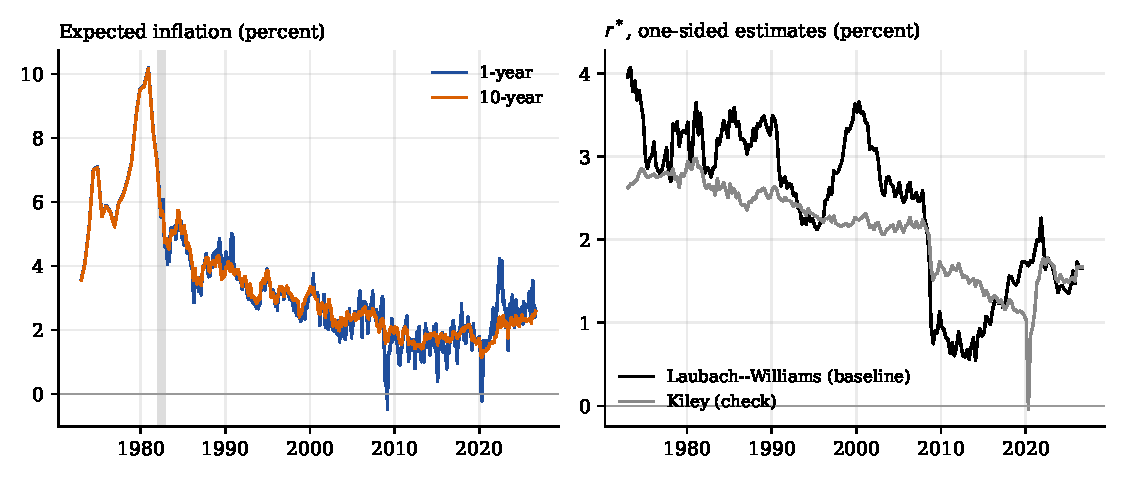
\includegraphics[width=\textwidth]{../replication/report/fig_inflation_rstar.pdf}
\caption{Expected Inflation and $r^*$}
\label{fig:infl}
\begin{flushleft}\footnotesize\textit{Notes:} Left: expected inflation, Livingston Survey before 1982 and Cleveland Fed model estimates after, shifted to the Cleveland level over 1982--84 and blended over 1982; shaded: the blending year. Right: one-sided, full-sample estimates of $\rs$ from the Laubach--Williams model (baseline) and Kiley's model (check). Percent.\end{flushleft}
\end{figure}

\textbf{Data.} All series are monthly averages from January 1973 to September 2026, from the public sources in Table~\ref{tab:data}. The BBB spread is Moody's Baa yield less the 10-year yield. Months in which the CPI and unemployment releases are missing (October 2025) are interpolated. The unemployment gap is the unemployment rate less the Congressional Budget Office's natural rate, placed in the middle month of each quarter and interpolated. Expected inflation is the Cleveland Fed's estimate at one and ten years from 1982 and the Livingston Survey's 12-month CPI expectation before, shifted to the Cleveland level by the mean difference over 1982--84 and blended over 1982. CAPE is Shiller's series spliced over 1990--92 in logs to the monthly average of a daily series. The real broad dollar is spliced in 2006 in logs, as are the nominal dollar and the S\&P 500.

\textbf{Market index.} Policy news is the first principal component of MP1, MP2, ED2, ED3 and ED4 in the monetary-event windows, scaled by its regression on the two-year yield change so that one unit moves the two-year yield by one percentage point. Unscheduled events with no change in MP1 and March--April 2020 are dropped. Each of the 10-year yield change, the S\&P 500 return and the dollar (DXY) return in the window is regressed on the factor. The residual covariance $\Sigma$ of the three regressions gives $w=\Sigma^{-1}\psi/(\psi'\Sigma^{-1}\psi)$. The S\&P 500 and DXY weights apply to 100 times the log of CAPE and of the real broad dollar, as percent changes in the window and in the index levels agree to first order. The weights bootstrap resamples announcements with replacement and recomputes the policy-news factor and the weights each time; draws use the seed in \texttt{lib/config.py}.

\textbf{FRB/US index.} The weights are the cumulative GDP responses at four quarters to a persistent unit shift in each variable, simulated in FRB/US with VAR-based expectations, divided by the response to a persistent one percentage point rise in the funds rate. The weight on the policy rate is its direct effect with expectations of future rates held fixed. House prices enter as 100 times the log of the price-to-rent ratio relative to its trailing 15-year average. The expenditure decomposition of Figure~\ref{fig:channels} uses the model's own identities for the components of GDP, weighted by their shares; it is run with the Board's FRB/US package and the data vintage of October 2026, downloaded by step 00 of the replication package.

\textbf{Policy-news definitions.} The two-year definition replaces the futures factor by the change in the two-year Treasury yield in the same window, with the same regressions and the same bootstrap of announcements. The Bauer--Swanson definition uses their surprise orthogonalized to public news \citep{bauer2023}, matched to this paper's announcements through 2019 and scaled so that one unit raises the two-year yield by one percentage point. The announcement bootstrap uses 5,000 draws for every weights-based interval; the block bootstraps of the outcome regressions use 500.

\textbf{Forecasting data.} The regressions use local projections of the 12-month-ahead change in the unemployment gap (four-quarter-ahead GDP growth) with HAC standard errors of 18 lags.

\begin{table}[tbp]\centering\small
\caption{Data Sources}\label{tab:data}
\begin{tabular}{p{0.38\textwidth}p{0.13\textwidth}p{0.42\textwidth}}\toprule
Series & Frequency & Source \\\midrule
Federal funds rate; 10-year yield; Baa yield; 30-year mortgage rate & Monthly & FRED FEDFUNDS, GS10, BAA, MORTGAGE30US \\
Real broad dollar; nominal broad dollar & Monthly & FRED RTWEXBGS, TWEXBPA; DTWEXBGS, TWEXBMTH (spliced in 2006) \\
CPI; CPI rent; Case--Shiller home prices; S\&P 500 & Monthly & FRED CPIAUCSL, CUUR0000SEHA, CSUSHPISA, SP500; Shiller's data before the FRED start \\
Unemployment rate; natural rate of unemployment; real GDP & Monthly; quarterly & FRED UNRATE; CBO, FRED NROU; GDPC1 \\
Expected inflation, 1 and 10 years & Monthly & Cleveland Fed, FRED EXPINF1YR, EXPINF10YR; before 1982, Livingston Survey (Philadelphia Fed) \\
$\rs$, Laubach--Williams & Quarterly & New York Fed, one-sided estimates \\
$\rs$, Kiley & Quarterly & One-sided estimates of the author \\
CAPE & Monthly & Shiller, spliced to the monthly average of a daily CAPE constructed by the repository's daily workflow \\
FRB/US simulations & Quarterly & Run for this paper's companion work with the public FRB/US package \\
Futures, yields, S\&P 500 and DXY in the window & Event & U.S.\ Monetary Policy Event-Study Database, ``monetary events'' \citep{acosta2025} \\
\bottomrule
\end{tabular}
\end{table}

\section{The Market Weights}\label{app:weights}
\subsection{Estimates and Precision}\label{sec:precision}
Table~\ref{tab:weights} gives the market weights under the baseline. A policy move that raises the two-year yield by one point raises the 10-year yield by \bl{psi:ten} points, lowers equity valuation by \bl{abs:psi:eq} percent and raises the real dollar by \bl{psi:usd} percent. Each asset carries a substantial part of the policy move, with shares of \bl{share:ten} for the 10-year yield, \bl{share:eq} for equity valuation and \bl{share:usd} for the dollar. The 90 percent intervals of the weights, from 5,000 bootstrap draws of the \bl{n:events} announcements, run from \bl{wb:ten:lo} to \bl{wb:ten:hi} for the 10-year yield, \bl{wb:eq:lo} to \bl{wb:eq:hi} for equity valuation and \bl{wb:usd:lo} to \bl{wb:usd:hi} for the dollar.

\begin{table}[tbp]\centering\small
\caption{Market Index: Responses to Policy News and Weights}\label{tab:weights}
\resizebox{\ifdim\width>\textwidth\textwidth\else\width\fi}{!}{%
\begin{tabular}{lrrrr}
\toprule
 & Response & Weight & 90\% interval & Share of policy move \\
\midrule
10-year Treasury yield (pp) & 0.53 (0.06) & 0.609 & [0.147, 1.114] & 0.33 \\
Equity valuation, 100 ln CAPE (percent) & $-$7.78 (0.93) & $-$0.051 & [$-$0.068, $-$0.030] & 0.40 \\
Real broad dollar, 100 ln (percent) & 4.22 (0.53) & 0.065 & [0.021, 0.112] & 0.28 \\
\bottomrule
\end{tabular}}
\begin{flushleft}\footnotesize\textit{Notes:} Announcement windows, 253 announcements, January 1996 to September 2026. Response: change in the window per unit of policy news, which moves the two-year yield by 1 percentage point (heteroskedasticity-robust standard errors in parentheses). Weight: one-factor generalized least squares, normalized so that the weights applied to the responses sum to 1. Interval: 5th and 95th percentiles of weights re-estimated on 5000 bootstrap samples of the announcements. Share: weight times response.\end{flushleft}
\end{table}


\subsection{Other Measures of Policy News and Event Samples}\label{sec:robother}
Table~\ref{tab:wvar} re-estimates the weights with the two-year yield and the Bauer--Swanson orthogonalized surprise as the measure of policy news, with announcements through 2019, and without the lower-bound years. The equity weight is \bl{wv:two:year:w:eq}, \bl{wv:to:2019:w:eq} and \bl{wv:no:lower:bound:w:eq} under the two-year yield and the two sample checks, and \bl{inf3:w:eq} under the Bauer--Swanson surprise, against \bl{w:eq} in the baseline. FRB/US gives the dollar more weight relative to equities than every one of these market calibrations.

\begin{table}[tbp]\centering\small
\caption{Weights Under Other Policy-News Series and Event Samples}\label{tab:wvar}
\resizebox{\ifdim\width>\textwidth\textwidth\else\width\fi}{!}{%
\begin{tabular}{lrrrrrrr}
\toprule
 & Events & $w$ 10-year & $w$ equities & $w$ dollar & $\psi$ 10-year & $\psi$ equities & $\psi$ dollar \\
\midrule
Baseline: Nakamura--Steinsson factor & 253 & 0.609 & $-$0.051 & 0.065 & 0.53 & $-$7.78 & 4.22 \\
Policy news is the 2-year yield change & 253 & 0.925 & $-$0.027 & 0.070 & 0.58 & $-$6.09 & 4.22 \\
Announcements through 2019 & 201 & 0.613 & $-$0.061 & 0.053 & 0.56 & $-$7.50 & 3.83 \\
No announcements December 2008--November 2015 & 197 & 0.986 & $-$0.039 & 0.058 & 0.49 & $-$7.82 & 3.69 \\
Policy news is the Bauer--Swanson orthogonalized surprise (to 2019) & 200 & 0.542 & $-$0.070 & 0.040 & 0.58 & $-$8.93 & 3.98 \\
\bottomrule
\end{tabular}}
\begin{flushleft}\footnotesize\textit{Notes:} Weights $w$ and responses $\psi$ as in Table~\ref{tab:weights}, re-estimated on each sample or with another policy-news measure: the window change of the two-year yield, or the surprise of \citet{bauer2023} orthogonalized to public news before the announcement, matched to this paper's announcements through 2019 and scaled so that one unit raises the two-year yield by one percentage point. In each case the weights applied to the responses sum to 1.\end{flushleft}
\end{table}



\subsection{Weights That Move}\label{sec:drift}
The weights define the unit, so I hold them fixed and show how they would drift. Re-estimating on an expanding window of announcements from 2006 keeps the 10-year and dollar weights inside the 90 percent band of the full-sample estimate at every date after 2010; the equity weight is outside the full-sample 90 percent bootstrap interval in \bl{exp:n} monthly estimates between \bl{exp:first} and \bl{exp:last}, by at most \bl{exp:post2010:min:eq} against a band edge of \bl{base:lo:eq} (Figure~\ref{fig:weightpath}). The overlapping monthly estimates are not \bl{exp:n} independent tests of instability. A 20-year rolling window fails after 2021, because it drops the announcements of 1996--2005. The 10-year weight is imprecise throughout. Apart from the equity weight in these years, the weights stay within their sampling error.

\begin{figure}[tbp]
\centering
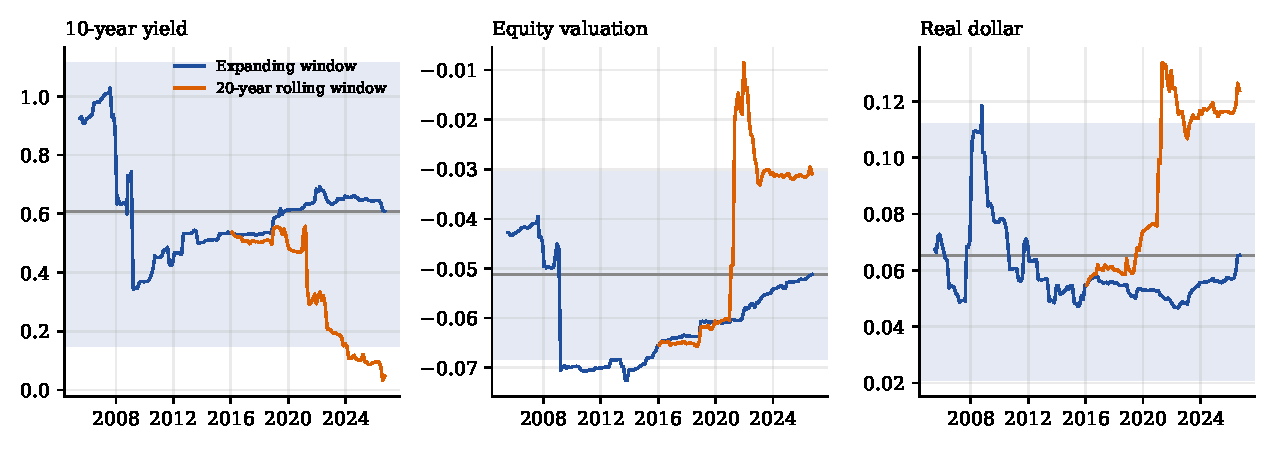
\includegraphics[width=\textwidth]{../replication/report/fig_weight_path.pdf}
\caption{The Weights on an Expanding and a Rolling Window}
\label{fig:weightpath}
\begin{flushleft}\footnotesize\textit{Notes:} Weights of the market index re-estimated on announcements to each date (expanding window, from the 80th announcement) and on the latest 20 years (rolling). Shaded: 90 percent bootstrap interval of the full-sample weights; the horizontal line is the full-sample weight.\end{flushleft}
\end{figure}

\end{appendices}
